\section{Общие положения}

\subsection{Цель, объект и предмет исследования}
\begin{frame}{Цель, объект и предмет исследования}
	\textbf{Целью} работы является совершенствование методов оценки параметров гармоник многотонального сигнала. \vspace{1em}

	\textbf{Объектом} исследования являются методы оценки параметров гармоник в силовых электрических сетях. \vspace{1em}
	
	\textbf{Предметом} исследования является точность и быстродействие численных методов оценки параметров гармоник.	
\end{frame}

\subsection{Задачи исследования}
\begin{frame}{Задачи исследования}
	\begin{enumerate}
		\item Анализ математических основ объекта исследования и формулировка математической модели многотонального сигнала.
		\item Изучение и экспериментальное исследование алгоритмов оценки параметров гармоник.
		\item Развитие математической модели многотональных сигналов в части расчета точности оценки амплитуды применительно к используемому при оценке параметров гармоник подходу, связанному с применением оконных функций.
		\item Разработка численных методов для оценки параметров гармоник, позволяющих достичь расчетной точности для амплитуды гармоники.
		\item Разработка алгоритмов для эффективного выполнения численных методов из предыдущей задачи.
		\item Разработка комплекса программа для анализа и доработки алгоритмов оценки параметров гармоник многотональных сигналов.
	\end{enumerate}
\end{frame}

\subsection{Научная новизна работы}
\begin{frame}{Научная новизна работы}
	\begin{enumerate}
		\item Дополнена математическая модель спектра многотонального сигнала  полученными и экспериментально проверенными формулами для нахождения границы Крамера-Рао при оценке амплитуды гармоники для взвешенного оконной функцией сигнала.
		\item Предложен численный метод нахождения оптимальной несмещенной оценки амплитуды гармоники на основе корреляционного анализа, а также предложена его быстрая реализация на основе алгоритмов разряженного БПФ.
		\item Реализован комплекс программ для экспериментальной проверки полученных в работе формул и анализа алгоритмов оценки параметров гармоник многотональных сигналов.
	\end{enumerate}	
\end{frame}

\subsection{Практическая значимость работы}
\begin{frame}{Практическая значимость работы}
	\begin{enumerate}
		\item Выведена формула для нахождения границы Крамера-Рао при применении оконной функции, которая позволяет повысить эффективность научных исследований различных алгоритмов обработки сигналов с применением оконных функций, заменив моделирование алгоритма с применением различных окон расчетом по предложенной формуле.
		\item Предложенный численный метод, вместе с его быстрой реализацией, позволяют повысить точность и достоверность результатов измерительных приборов для электрических сетей.
		\item Разработанный комплекс программ позволяет проводить научные исследования в области цифровой обработки сигналов и используется в учебном процессе.
	\end{enumerate}
\end{frame}

\section{Математическая модель многотонального сигнала}
\subsection{Ограничение ДПФ}
\begin{frame}{Ограничение ДПФ}
	\textsc{Рисунок, на котором показана проблема нахождения гармоники сигнала с частотой, находящейся между дискретными гармониками ДПФ.}
\end{frame}

\begin{frame}{Виляние оконной функции}
	\textsc{Рисунок, показывающий, что происходит со спектром гармоники при наложении на него окна. Лучше в двух частях - с прямоугольным окном и окном Кайзера.}	
\end{frame}

\begin{frame}{Методы интерполирования спектра}
	\textsc{Справа - поясняющий рисунок и формулы, слева - список основных методов.
	Можно взять из диссертации Елизарова.}	
\end{frame}

\begin{frame}{Методы экстраполирования сигнала}
	\begin{minipage}[t]{0.47\linewidth}
		\centering 
		\textbf{Сигнал (частота=5.2)}
		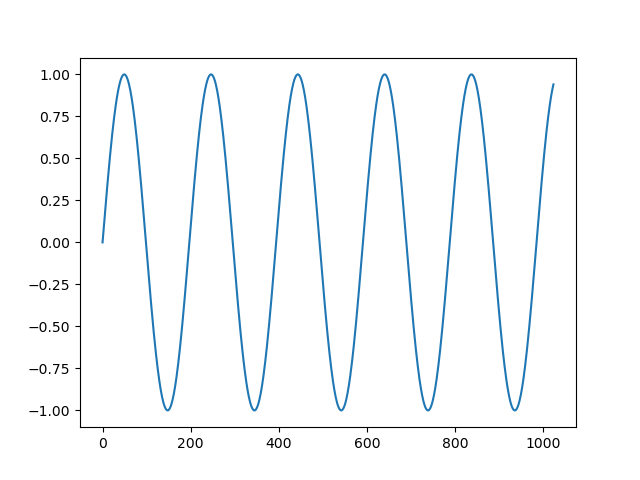
\includegraphics[width=.9\linewidth]{signal}
		\textbf{Экстраполированный сигнал }
		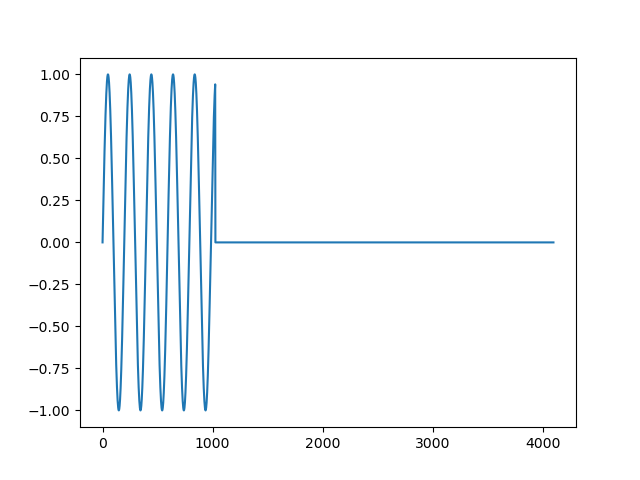
\includegraphics[width=.9\linewidth]{interpolated_signal}		
	\end{minipage}
	\hfill
	\begin{minipage}[t]{0.47\linewidth}
		\centering 
		\textbf{Спектр}
		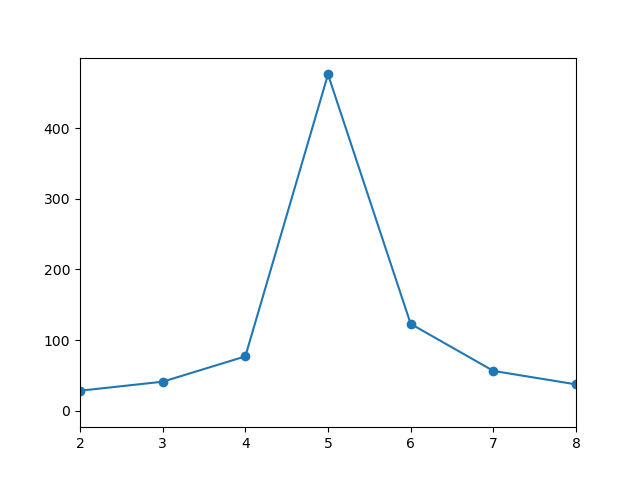
\includegraphics[width=.9\linewidth]{spectrum}
		\textbf{Спектр экстр. сигнала}
		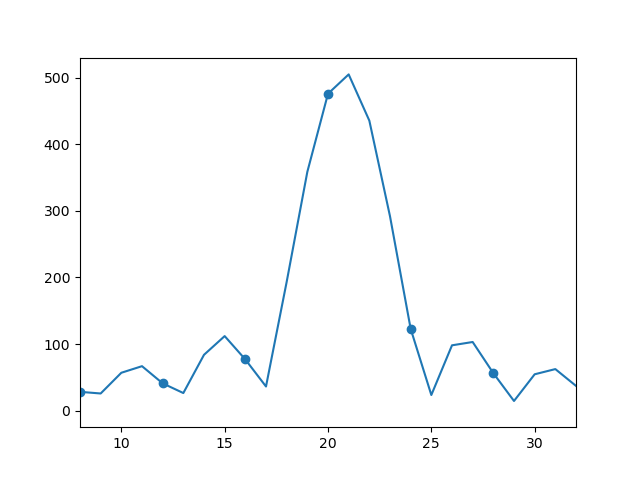
\includegraphics[width=.9\linewidth]{spectrum_of_interpolated_signal}
	\end{minipage}
\end{frame}

\subsection{Граница Крамера-Рао}
\begin{frame}{Теоретическая точность определения амплитуды гармоник}
	\textsc{Формулы для границы Крамера-Рао для амплитуды гармоник.}
\end{frame}
\note{Привести ссылку на статью в Скопус}


\begin{frame}{Практическая точность методов}
	\textsc{Рисунки по точности методов с границей.
	Где-то строили такие графики. Можно взять у Димы.}
\end{frame}

\subsection{Уточнение границы Крамера-Рао}
\begin{frame}{Оценка дисперсии амплитуды гармоники}
	\textsc{Основные результаты из статьи}
\end{frame}

\begin{frame}{Экспериментальная проверка формулы для оценки дисперсии}
	\textsc{Графики из статьи}
\end{frame}

\begin{frame}{Дополненная математическая модель многотонального сигнала}
    \begin{center}
		\Large
		Математическая модель многотонального сигнала для оценки параметров гармоник
	\end{center}	
	\begin{itemize}
		\item Математическое описание свойств ДПФ.
		\item Математическое описание влияния оконных функций.
		\item \textbf{Формулы для оценки дисперсии результатов измерений}.
	\end{itemize}
\end{frame}

\section{Анализ многотональных сигналов}

\subsection{Нахождение гармоники сигнала}
\begin{frame}{Интерполирование спектра}
	\textsc{Слева - прямое интерполирование, справа - метод корреляционных функций}
\end{frame}

\begin{frame}{Двойное интерполирование сигнала и спектра}
	\textsc{Рисунок и формулы напишу чуть позже.}
\end{frame}

\begin{frame}{Интерполирование сигнала для оценки параметров гармоник}
	\textsc{Рисунок и формулы напишу чуть позже.}
\end{frame}

\begin{frame}{Сравнение корреляционных методов}
	\begin{tabular}{llll}
		\toprule Интерполирование: &
		спектра & 
		двойное &
		сигнала\\ 
		\midrule
		Точность &
		Не высокая & 
		Высокая &
		Наивысшая\\ 
		\midrule
		Быстродействие &
		Высокое & 
		Среднее &
		Низкое \\ 
		\midrule		
	\end{tabular}
\end{frame}

\subsection{Поиск гармоник}
\begin{frame}{Алгоритм поиска гармоник}
	\textsc{ГСА алгоритма поиска гармоник из зарегистрированной программы}
\end{frame}

\begin{frame}{Расчет гармоник и интергармоник}
	\textsc{Свидетельство о регистрации программы}
\end{frame}

\subsection{Практическая реализация}
\begin{frame}{Библиотека SFFT}
	
\end{frame}

\begin{frame}{Разряженное FFT}
	
\end{frame}

\section{Заключение}

\subsection{Результаты работы}
\begin{frame}{Результаты работы}
	По результатам работы опубиковано ...
\end{frame}

\subsection{Основные положения выносимые на защиту}
\begin{frame}{Основные положения выносимые на защиту}
	\begin{enumerate}
		\item Дополнение к математической модели многотонального сигнала в виде формулы, позволяющей определить дисперсию оценки амплитуды гармоники, отличающемуся от известной границы Крамера-Рао учетом изменения дисперсии после применения оконных функций.
		\item Основанный на корреляционном анализе численный метод, позволяющий определить параметры гармоник сигналов с точностью, определяемой уточненной границей Крамера-Рао, включающий в себя вычислительно-эффективную схему расчета корреляций и отличающийся от известных методов отсутствием потерь в точности результатов при интерполировании параметров гармоник.
		\item Комплекс программ для анализа и построения алгоритмов оценки параметров многотональных сигналов.
	\end{enumerate}
\end{frame}

